\section{Results}\label{sec:results}

All numbers in this section are generated directly from the campaign's raw telemetry
(\S\ref{sec:method}); none is hand-typed, and Appendix~\ref{app:claims} traces every claim to its
generating script. \NRunsTotal{} runs completed across the three arms with zero
aborted runs and zero token-ceiling breaches. Analysis's provenance check found $\NProvenanceProblems{}$
deviation across the merged arms --- the campaign's supervisor was restarted mid-run after a host
infrastructure failure unrelated to the experiment (Appendix~\ref{app:deviations}, D-104m); the fix
that shipped with the restart touched only the supervisor's own health check, never the code on the
execution path of a run, which we verified by diff before treating the arms as one dataset (D-104n).

\subsection{Does the full agent system beat static orchestration?}

Table~\ref{tab:main} gives medians with interquartile ranges for every configuration; Table~\ref{tab:effects}
gives the paired comparison against \texttt{baseline} for every metric, with bootstrap confidence
intervals on the median difference, Cliff's $\delta$ with its own bootstrap interval, and a
Holm-corrected Mann--Whitney $p$-value. Figure~\ref{fig:mttr} shows the full recovery-time
distributions and Figure~\ref{fig:effects} the effect sizes across metrics as a forest plot.

\begin{table}[t]
\centering
\caption{Medians [IQR] per configuration, $n$ replicates pooled across scenarios.}
\label{tab:main}
\small
\begin{tabular}{llrrrrr}
\toprule
config & LLM & $n$ & MTTR (s) & cost & manual interv. & decision correct \\
\midrule
baseline & none & 80 & 378 [244] & 158 [113] & 1.00 [0] & 0 [0] \\
rule\_based & none & 80 & 30.0 [15.9] & 158 [113] & 0 [0.250] & 0 [0] \\
autoscale & none & 80 & 52.4 [359] & 82.5 [122] & 0.500 [1.00] & 0 [0] \\
monitor\_only & live & 40 & 359 [210] & 1{,}223 [525] & 1.00 [1.00] & 0 [0] \\
recovery\_only & live & 40 & 220 [75.0] & 1{,}223 [630] & 6.00 [1.00] & 0 [0] \\
optimization\_only & live & 40 & 267 [360] & 76.5 [128] & 1.00 [1.00] & 0 [0.250] \\
schema\_only & live & 40 & 315 [353] & 920 [122] & 1.00 [1.25] & 0 [0.250] \\
full & live & 80 & 235 [143] & 69.8 [35.1] & 6.00 [8.00] & 0 [1.00] \\
\bottomrule
\end{tabular}

\end{table}

\begin{table}[t]
\centering
\caption{Effect of each configuration against \texttt{baseline}: bootstrap 95\% CI on the median
  difference, Cliff's $\delta$ with its own 95\% CI, and the Holm-corrected Mann--Whitney $p$-value
  ($^{*}p_{\mathrm{Holm}}<0.05$).}
\label{tab:effects}
\scriptsize
\begin{tabular}{llrrr}
\toprule
config & metric & $\Delta$ median [95\% CI] & Cliff's $\delta$ [95\% CI] & $p_{\mathrm{Holm}}$ \\
\midrule
rule\_based & MTTR (s) & \ensuremath{-}348 [\ensuremath{-}419, \ensuremath{-}303] & \ensuremath{-}0.73 [\ensuremath{-}0.85, \ensuremath{-}0.60] & <0.001$^{*}$ \\
autoscale & MTTR (s) & \ensuremath{-}326 [\ensuremath{-}406, \ensuremath{-}82.7] & \ensuremath{-}0.49 [\ensuremath{-}0.63, \ensuremath{-}0.32] & <0.001$^{*}$ \\
monitor\_only & MTTR (s) & \ensuremath{-}19.2 [\ensuremath{-}99.6, 59.8] & \ensuremath{-}0.09 [\ensuremath{-}0.32, 0.13] & 1.000 \\
recovery\_only & MTTR (s) & \ensuremath{-}159 [\ensuremath{-}229, \ensuremath{-}105] & \ensuremath{-}0.70 [\ensuremath{-}0.83, \ensuremath{-}0.55] & <0.001$^{*}$ \\
optimization\_only & MTTR (s) & \ensuremath{-}111 [\ensuremath{-}188, 15.9] & \ensuremath{-}0.27 [\ensuremath{-}0.50, \ensuremath{-}0.025] & 0.134 \\
schema\_only & MTTR (s) & \ensuremath{-}63.1 [\ensuremath{-}182, 87.4] & \ensuremath{-}0.19 [\ensuremath{-}0.42, 0.056] & 0.638 \\
full & MTTR (s) & \ensuremath{-}143 [\ensuremath{-}212, \ensuremath{-}94.7] & \ensuremath{-}0.56 [\ensuremath{-}0.70, \ensuremath{-}0.42] & <0.001$^{*}$ \\
rule\_based & cost (units) & 0 [0, 0] & 0.00 [\ensuremath{-}0.14, 0.14] & 1.000 \\
autoscale & cost (units) & \ensuremath{-}75.0 [\ensuremath{-}75.0, \ensuremath{-}75.0] & \ensuremath{-}0.62 [\ensuremath{-}0.76, \ensuremath{-}0.45] & <0.001$^{*}$ \\
monitor\_only & cost (units) & 1{,}065 [1{,}065, 1{,}074] & 1.00 [1.0, 1.0] & <0.001$^{*}$ \\
recovery\_only & cost (units) & 1{,}065 [1{,}065, 1{,}389] & 1.00 [1.0, 1.0] & <0.001$^{*}$ \\
optimization\_only & cost (units) & \ensuremath{-}81.0 [\ensuremath{-}81.0, \ensuremath{-}48.3] & \ensuremath{-}0.47 [\ensuremath{-}0.72, \ensuremath{-}0.20] & <0.001$^{*}$ \\
schema\_only & cost (units) & 763 [750, 763] & 1.00 [1.0, 1.0] & <0.001$^{*}$ \\
full & cost (units) & \ensuremath{-}87.7 [\ensuremath{-}96.2, \ensuremath{-}87.7] & \ensuremath{-}0.66 [\ensuremath{-}0.81, \ensuremath{-}0.51] & <0.001$^{*}$ \\
rule\_based & manual interv. & \ensuremath{-}1.00 [\ensuremath{-}1.00, \ensuremath{-}1.00] & \ensuremath{-}0.75 [\ensuremath{-}0.85, \ensuremath{-}0.65] & <0.001$^{*}$ \\
autoscale & manual interv. & \ensuremath{-}0.500 [\ensuremath{-}1.00, 0] & \ensuremath{-}0.50 [\ensuremath{-}0.61, \ensuremath{-}0.39] & <0.001$^{*}$ \\
monitor\_only & manual interv. & 0 [0, 0] & 0.28 [0.15, 0.42] & <0.001$^{*}$ \\
recovery\_only & manual interv. & 5.00 [5.00, 5.50] & 0.97 [0.93, 1.0] & <0.001$^{*}$ \\
optimization\_only & manual interv. & 0 [0, 1.00] & 0.20 [\ensuremath{-}0.050, 0.42] & 0.121 \\
schema\_only & manual interv. & 0 [0, 0] & 0.25 [0.12, 0.38] & <0.001$^{*}$ \\
full & manual interv. & 5.00 [5.00, 8.00] & 0.79 [0.70, 0.88] & <0.001$^{*}$ \\
rule\_based & decision correct & 0 [0, 0] & 0.00 [0, 0] & 1.000 \\
autoscale & decision correct & 0 [0, 0] & 0.00 [0, 0] & 1.000 \\
monitor\_only & decision correct & 0 [0, 0] & 0.00 [0, 0] & 1.000 \\
recovery\_only & decision correct & 0 [0, 0] & 0.00 [0, 0] & 1.000 \\
optimization\_only & decision correct & 0 [0, 0] & 0.25 [0.12, 0.38] & <0.001$^{*}$ \\
schema\_only & decision correct & 0 [0, 0] & 0.25 [0.12, 0.38] & <0.001$^{*}$ \\
full & decision correct & 0 [0, 1.00] & 0.42 [0.31, 0.54] & <0.001$^{*}$ \\
\bottomrule
\end{tabular}

\end{table}

\begin{figure}[t]
\centering
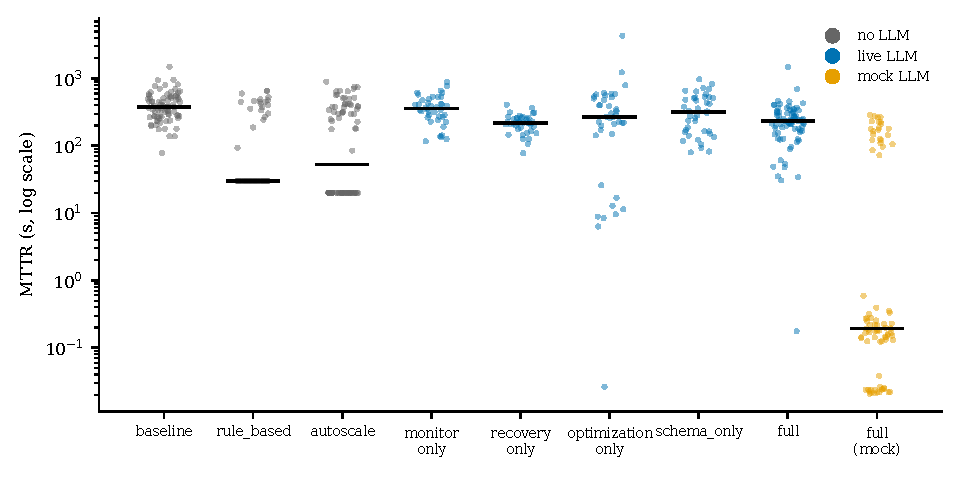
\includegraphics[width=0.75\linewidth]{generated/fig_mttr.pdf}
\caption{Recovery-time distribution by configuration (log scale).}
\label{fig:mttr}
\end{figure}

\begin{figure}[t]
\centering
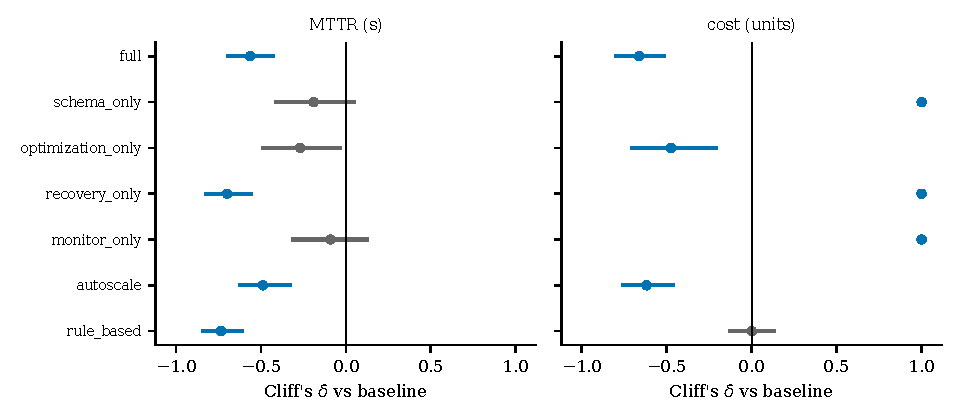
\includegraphics[width=0.95\linewidth]{generated/fig_effects.pdf}
\caption{Cliff's $\delta$ against \texttt{baseline}, by configuration and metric, with bootstrap 95\%
  intervals.}
\label{fig:effects}
\end{figure}

\texttt{full} reduces MTTR from \NMttrBaselineMedian{}\,s to \NMttrFullMedian{}\,s
($\Delta=\NDiffMttrSFull{}$\,s, $\NRelpctMttrSFull{}$\%, Cliff's $\delta=\NDeltaMttrSFull{}$,
$p_{\mathrm{Holm}}\NPHolmMttrSFull{}$) and cost from \NCostBaselineMedian{} to \NCostFullMedian{} units
($\NRelpctCostUnitsFull{}$\%, $\delta=\NDeltaCostUnitsFull{}$, $p_{\mathrm{Holm}}\NPHolmCostUnitsFull{}$).
Both are real, significant effects, but the MTTR reduction is well short of the $\sim$45\% the
replicated paper reports and far short of the $\sim$100\% a mock evaluation of the same configuration
implies (\S\ref{sec:livemock}). The cost result is the one headline claim that survives at a similar or
larger magnitude than reported --- with the caveat, quantified in \S\ref{sec:sensitivity}, that it
depends on the assumed provisioning gap between static and right-sized allocation.

Manual interventions do \emph{not} fall under \texttt{full}: the median rises from
\NIntervBaselineMedian{} to \NIntervFullMedian{} ($\Delta=\NDiffManualInterventionsFull{}$,
$\NRelpctManualInterventionsFull{}$\%, $\delta=\NDeltaManualInterventionsFull{}$,
$p_{\mathrm{Holm}}\NPHolmManualInterventionsFull{}$), the opposite direction from the replicated
paper's reported reduction of over 70\%. \texttt{recovery\_only} shows the same rise
($\NRelpctManualInterventionsRecoveryOnly{}$\%). Because \texttt{baseline} escalates exactly once per
injected fault by construction (D-044), and an agent configuration can propose, be rate-limited or
budget-denied, and re-propose on a later tick of the same 300\,s loop, each such cycle can add its own
escalation; we did not instrument which of these mechanisms dominates, so we report the measurement
and flag the mechanism as open (\S\ref{sec:discussion}). Whatever the mechanism, a system whose central
claim is fewer manual interventions increasing them on this metric is a result the paper reports
plainly rather than reconciles away.

\subsection{Is the full system better than cheap, non-agent automation?}

\texttt{rule\_based} and \texttt{autoscale} make no model call and cost nothing per run beyond the
static infrastructure. On MTTR both beat every agent configuration, including \texttt{full}:
\texttt{rule\_based} reaches \NMttrRuleBasedMedian{}\,s ($\NRelpctMttrSRuleBased{}$\% vs.\ baseline,
$\delta=\NDeltaMttrSRuleBased{}$) and \texttt{autoscale} \NMttrAutoscaleMedian{}\,s
($\NRelpctMttrSAutoscale{}$\%, $\delta=\NDeltaMttrSAutoscale{}$), against \texttt{full}'s
$\NRelpctMttrSFull{}$\%. Both also reduce or leave unchanged manual interventions
(\NRelpctManualInterventionsRuleBased{}\% and \NRelpctManualInterventionsAutoscale{}\%), where
\texttt{full} increases them. \texttt{autoscale} reduces cost by \NRelpctCostUnitsAutoscale{}\%,
narrower than \texttt{full}'s \NRelpctCostUnitsFull{}\%; \texttt{rule\_based}, which does not
right-size, shows no cost effect ($\NRelpctCostUnitsRuleBased{}$\%, $p_{\mathrm{Holm}}=\NPHolmCostUnitsRuleBased{}$),
as designed (D-058). Neither comparator can execute an accepted mitigation by construction
(\texttt{decision\_correct}$=0$, D-059), which is the one axis \texttt{full} wins outright
(\S\ref{sec:decision}). On speed and on manual-intervention count, at these fault scenarios and this
control-loop timing, cheap deterministic automation beats the LLM-driven system it was built to be
compared against; this is the sharpest instance of D-058's design intent (``do agents beat cheap
automation too?'') returning a plain no on two of four metrics.

\subsection{Decision quality}\label{sec:decision}

\texttt{decision\_correct} is scored against a per-scenario accepted-mitigation set
(\S\ref{sec:method}); non-agent configurations score zero by construction. Among agent configurations,
only \texttt{full} ($\delta=\NDeltaDecisionCorrectFull{}$, $p_{\mathrm{Holm}}\NPHolmDecisionCorrectFull{}$),
\texttt{optimization\_only} ($\delta=\NDeltaDecisionCorrectOptimizationOnly{}$) and
\texttt{schema\_only} ($\delta=\NDeltaDecisionCorrectSchemaOnly{}$) move the metric significantly;
\texttt{monitor\_only} and \texttt{recovery\_only} do not. Because Cliff's $\delta$ against an
all-zero comparator is exactly the treatment group's success rate, these $\delta$ values are read
directly as correct-mitigation rates: \texttt{full} executes an accepted mitigation in
$\NDeltaDecisionCorrectFull{}$ of its runs. This is the one metric on which the live agent system does
something no static or rule-based comparator can claim to do at all, and it is also the metric
furthest from the mock evaluation's answer of \NLiveVsMockDecisionCorrectMock{} (\S\ref{sec:livemock}).

\subsection{Per-scenario heterogeneity}

\begin{table}[t]
\centering
\caption{Median MTTR (s) by configuration and scenario.}
\label{tab:scenarios}
\small
\begin{tabular}{lrrrr}
\toprule
config & ingress\_burst & resource\_contention & schema\_drift & upstream\_delay \\
\midrule
baseline & 352 & 386 & 424 & 353 \\
rule\_based & 30.0 & 30.0 & 433 & 30.0 \\
autoscale & 20.0 & 20.0 & 363 & 393 \\
monitor\_only & 366 & 412 & 320 & 275 \\
recovery\_only & 223 & 183 & 224 & 248 \\
optimization\_only & 10.5 & 267 & 502 & 281 \\
schema\_only & 453 & 343 & 120 & 553 \\
full & 148 & 318 & 214 & 237 \\
\bottomrule
\end{tabular}

\end{table}

\begin{figure}[t]
\centering
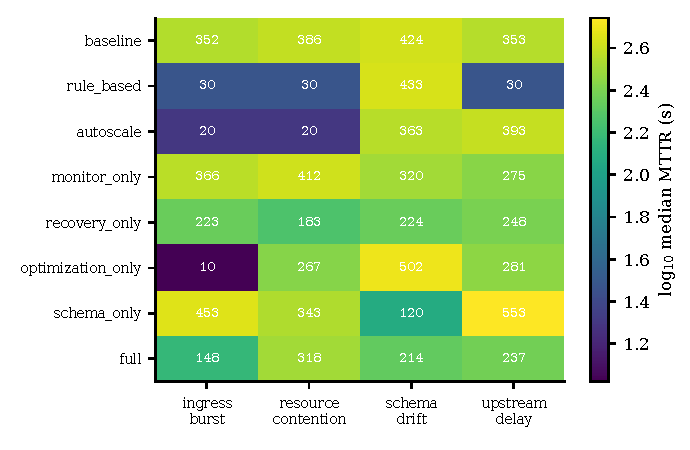
\includegraphics[width=0.85\linewidth]{generated/fig_scenarios.pdf}
\caption{MTTR by configuration and scenario.}
\label{fig:scenarios}
\end{figure}

Table~\ref{tab:scenarios} and Figure~\ref{fig:scenarios} break MTTR down by (configuration, scenario).
No configuration dominates every scenario. \texttt{optimization\_only} is fastest on
\texttt{ingress\_burst} but slower than \texttt{baseline} on \texttt{schema\_drift}, a fault type its
one enabled non-monitoring agent cannot act on; \texttt{schema\_only} shows the mirror pattern. This is
the expected shape of a single-agent ablation --- an agent helps on the fault type it owns and is
inert, or adds pure overhead, elsewhere --- and it argues against reading any single scenario's number
as the configuration's general behaviour.

\subsection{Mock versus live: the central methodological finding}\label{sec:livemock}

\begin{table}[t]
\centering
\caption{\texttt{full}, live model vs.\ deterministic mock, otherwise identical configuration and
  scenarios; Cliff's $\delta$ with 95\% CI, Holm-corrected $p$.}
\label{tab:live_mock}
\small
\begin{tabular}{lrrrr}
\toprule
metric & live & mock & Cliff's $\delta$ [95\% CI] & $p_{\mathrm{Holm}}$ \\
\midrule
MTTR (s) & 235 & 0.193 & 0.81 [0.72, 0.90] & <0.001 \\
cost (units) & 69.8 & 833 & -0.82 [-0.92, -0.71] & <0.001 \\
manual interv. & 6.00 & 0 & 0.87 [0.79, 0.93] & <0.001 \\
decision correct & 0 & 1.00 & -0.57 [-0.69, -0.46] & <0.001 \\
freshness (s) & 14.0 & 0.0801 & 0.25 [0.074, 0.42] & 0.004 \\
\bottomrule
\end{tabular}

\end{table}

\begin{figure}[t]
\centering
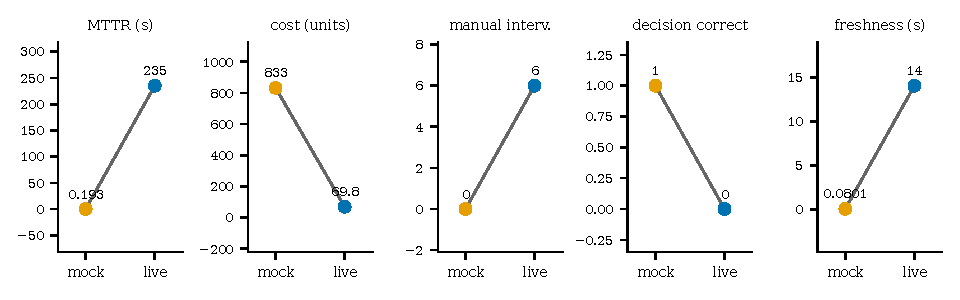
\includegraphics[width=0.95\linewidth]{generated/fig_live_mock.pdf}
\caption{\texttt{full}, live vs.\ mock, per metric (median). Linear axes deliberately: two metrics are
  exactly zero for one arm, which a shared log axis cannot represent.}
\label{fig:live_mock}
\end{figure}

Table~\ref{tab:live_mock} and Figure~\ref{fig:live_mock} compare \texttt{full} run identically except
for the model: arm A (live)
against arm C (the same configuration, deterministic mock); effect sizes and Holm-corrected
$p$-values for every metric are in the table. MTTR falls from \NLiveVsMockMttrSLive{}\,s live to
\NLiveVsMockMttrSMock{}\,s mock; decision-correct rises from \NLiveVsMockDecisionCorrectLive{} to
\NLiveVsMockDecisionCorrectMock{}; manual interventions fall from \NLiveVsMockManualInterventionsLive{}
to \NLiveVsMockManualInterventionsMock{}; freshness falls from \NLiveVsMockFreshnessSLive{}\,s to
\NLiveVsMockFreshnessSMock{}\,s. Cost moves the other way, live cheaper than mock
(\NLiveVsMockCostUnitsLive{} vs.\ \NLiveVsMockCostUnitsMock{} units) --- consistent with the
provisioning term (D-061) dominating over a control loop so short that the mock resolves the fault
almost before the loop has run long enough to accrue right-sizing benefit; we report this as measured
without a stronger causal claim. Read together with \S\ref{sec:decision}, a mock evaluation of this
system is not a scaled-down or noisier version of the live evaluation; on recovery time and decision
quality it is a categorically different, far more favourable experiment. Any claim made from a mock
run about this class of system should be read as a claim about the mock, not about the model.

\subsection{LLM accounting}

\begin{table}[t]
\centering
\caption{LLM accounting per agent configuration, counted at the moment a call is or is not made
  (\S\ref{sec:method}).}
\label{tab:llm}
\small
\begin{tabular}{lrrrrrrr}
\toprule
config & calls & cache hits & degraded & invalid & API tokens & latency (s) & degraded \% \\
\midrule
monitor\_only & 1.00 & 143 & 0 & 0 & 1{,}244 & 4.37 & 0\% \\
recovery\_only & 2.00 & 262 & 0 & 0 & 2{,}737 & 10.5 & 0\% \\
optimization\_only & 2.00 & 258 & 0 & 0 & 2{,}998 & 9.22 & 0\% \\
schema\_only & 2.00 & 274 & 0 & 0 & 2{,}550 & 5.73 & 0\% \\
full & 4.00 & 214 & 0 & 0 & 5{,}946 & 15.0 & 0\% \\
\bottomrule
\end{tabular}

\end{table}

Table~\ref{tab:llm} reports real model calls, cache hits, degraded proposals, invalid outputs, tokens
and latency per agent configuration, counted at the moment a call is or is not made
(\S\ref{sec:method}). Across the campaign, degraded and invalid rates are both zero: no budget
exhaustion, no provider-unavailable episode, and no schema-invalid output survived into the final
runs. This is a property of \emph{this} campaign, not a guarantee; the pilot that preceded it did find
a live cache-poisoning defect (Appendix~\ref{app:deviations}, D-104l) that the accounting exists to
catch, fixed before the campaign, not during it.

\subsection{Sensitivity}\label{sec:sensitivity}

\begin{table}[t]
\centering
\caption{Closed-form break-even points: the assumed human-latency median (s) and static provisioning
  (units) at which each configuration stops beating its comparator.}
\label{tab:sensitivity}
\small
\begin{tabular}{lrrrr}
\toprule
config & MTTR (s) & human break-even (s) & cost reduction (\%) & static break-even \\
\midrule
autoscale & 52.4 & 49.9 & 47.6 & 3.00 \\
full & 235 & 224 & 55.7 & 2.15 \\
monitor\_only & 359 & 342 & -676 & -- \\
optimization\_only & 267 & 254 & 51.4 & 2.60 \\
recovery\_only & 220 & 209 & -676 & -- \\
rule\_based & 30.0 & 28.5 & 0 & -- \\
schema\_only & 315 & 300 & -484 & -- \\
\bottomrule
\end{tabular}

\end{table}

\begin{figure}[t]
\centering
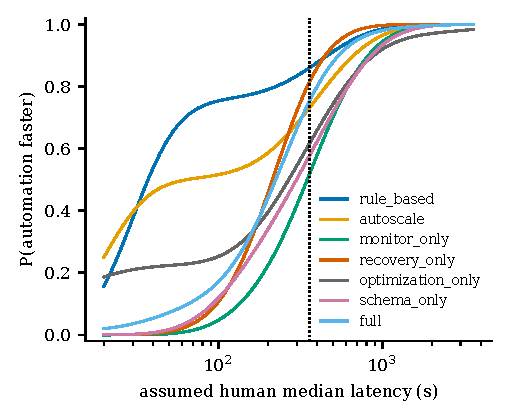
\includegraphics[width=0.75\linewidth]{generated/fig_human_sensitivity.pdf}
\caption{$P(\text{automation faster than the simulated human})$ as a function of the assumed human
  median latency.}
\label{fig:human_sensitivity}
\end{figure}

\begin{figure}[t]
\centering
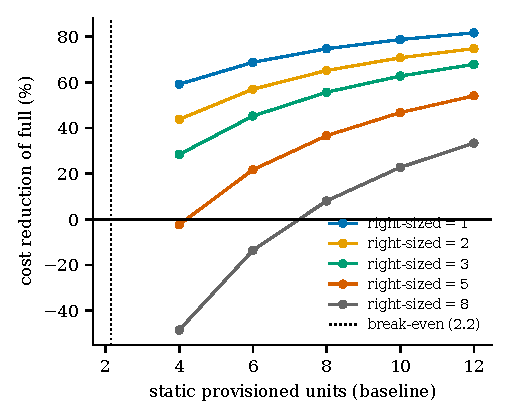
\includegraphics[width=0.75\linewidth]{generated/fig_cost.pdf}
\caption{\texttt{full}'s cost reduction as a function of the assumed static provisioning level.}
\label{fig:cost}
\end{figure}

Table~\ref{tab:sensitivity} and Figures~\ref{fig:human_sensitivity}--\ref{fig:cost} give the two
closed-form sensitivities described in \S\ref{sec:method}. \texttt{full} beats the simulated human
baseline down to a human median latency of \NBreakEvenHumanFull{}\,s, well below the assumed
\NHumanMedian{}\,s but far above \texttt{rule\_based}'s break-even of \NBreakEvenHumanRuleBased{}\,s ---
\texttt{rule\_based}'s speed advantage is robust to a much faster assumed on-call than \texttt{full}'s
is. On the cost side, \texttt{full}'s reduction claim holds down to a static provisioning assumption of
\NBreakEvenStaticFull{} units; below that, a baseline that is not badly over-provisioned in the first
place erases the saving. Both sensitivities make the same point as \S\ref{sec:livemock} from a
different angle: the headline numbers are conditional on modelling choices, and we give the reader the
condition rather than only the number.

\subsection{Adversarial containment}

\begin{table}[t]
\centering
\caption{Adversarial corpus graded against the independent specification oracle, by category.}
\label{tab:adversarial}
\scriptsize
\begin{tabular}{lrllll}
\toprule
category & cases & containment [Wilson 95\%] & over-block & oracle agreement & fail-open \\
\midrule
boundary\_grid & 4320 & 3056/3056 [0.9987, 1.0000] & 0/1264 [0.0000, 0.0030] & 4320/4320 [0.9991, 1.0000] & 0 \\
defense\_in\_depth & 133 & 133/133 [0.9719, 1.0000] & -- & 133/133 [0.9719, 1.0000] & 0 \\
fuzz & 1000 & 606/606 [0.9937, 1.0000] & 0/394 [0.0000, 0.0097] & 1000/1000 [0.9962, 1.0000] & 0 \\
injection & 28 & 28/28 [0.8794, 1.0000] & -- & 28/28 [0.8794, 1.0000] & 0 \\
param\_extremes & 66 & 44/44 [0.9197, 1.0000] & 0/22 [0.0000, 0.1487] & 66/66 [0.9450, 1.0000] & 0 \\
\textbf{overall} & 5547 & 3867/3867 [0.9990, 1.0000] & 0/1680 [0.0000, 0.0023] & 5547/5547 [0.9993, 1.0000] & 0 \\
\bottomrule
\end{tabular}

\end{table}

Table~\ref{tab:adversarial} grades the generated corpus (\S\ref{sec:method}) against the independent
specification oracle, by category and overall. Overall containment is
\NAdversarialContained{}/\NAdversarialUnsafe{} ($\geq\NAdversarialWilsonLo{}$, Wilson 95\%), the
over-block rate on legal, non-unsafe proposals is zero (Table~\ref{tab:adversarial} gives the exact
denominator) and exact agreement with the oracle across all \NAdversarialCases{} graded cases is 100\%,
with \NAdversarialGateErrors{} gate errors. This is
measured \emph{after} the two contract-layer fixes L6(i)--(ii) found by an earlier pass of the same
corpus (\S\ref{sec:lessons}); the number here is a property of the fixed system, and the corpus that
found the gap is now committed as a regression test against exactly this claim.
